\documentclass{standalone}
\usepackage{tikz}
\usetikzlibrary{shapes.geometric, arrows}

\definecolor{mycolor}{RGB}{0, 153, 255}
\tikzstyle{process} = [rectangle, rounded corners,
                       minimum width=2cm, minimum height=1cm,
                       text centered, draw=black, fill=mycolor,
                       text=white, line width=0.3mm]

\tikzstyle{arrow} = [thick,->,>=stealth]

\begin{document}
    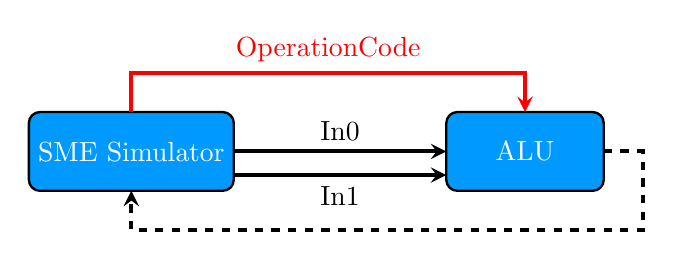
\begin{tikzpicture}[node distance=2cm]
        
        \node (Simulator) [process] {SME Simulator};
        
        
        %AND Gates
        \node (AND0) [process, right of = Simulator, xshift=3cm, yshift=0cm] {ALU};
        

        %Lines to ALU gate
        \draw [arrow, line width=0.5mm] (1.3,0) -- node [above] {In0} (4,0);
        \draw [arrow, line width=0.5mm] (1.3,-0.3) -- node [below] {In1} (4,-0.3);
        \draw [arrow, line width=0.5mm, color=red] (0,0.5) --  (0,1) -- node [above] {OperationCode} (5,1) -- (5,0.5) ;
        
        %Output line to simulator
        %AND3
        \draw [arrow, line width=0.5mm, dashed] (6,0) -- ++(0.5, 0) -- ++(0,-1) -- ++(-6.5,0) -- (0,-0.5);
        
    
    \end{tikzpicture}
\end{document}
